\documentclass[twocolumn,a4j]{jsarticle}
\setlength{\topmargin}{-18.5cm}
\setlength{\oddsidemargin}{-8.5mm}
\setlength{\evensidemargin}{-8.5mm}
\setlength{\textwidth}{19cm}
\setlength{\textheight}{26.5cm}

\usepackage[top=15truemm,bottom=20truemm,left=20truemm,right=20truemm]{geometry}
\usepackage[latin1]{inputenc}
\usepackage{amsmath}
\usepackage{amsfonts}
\usepackage{amssymb}
\usepackage[dvipdfmx]{graphicx}
\usepackage[hang,small,bf]{caption}
\usepackage[subrefformat=parens]{subcaption}
\usepackage[dvipdfmx]{color}
\usepackage{listings}
\usepackage{listings,jvlisting}
\usepackage{geometry}
\usepackage{framed}
\usepackage{color}
\usepackage[dvipdfmx]{hyperref}
\usepackage{ascmac}
\usepackage{enumerate}
\usepackage{tabularx}
\usepackage{cancel}
\usepackage{scalefnt}
\usepackage{overcite}
\usepackage{otf}
\usepackage{multicol}
\usepackage[geometry]{ifsym}

% キャプション後ろのダブルコロンを消す
\makeatletter
\long\def\@makecaption#1#2{%
  \vskip\abovecaptionskip
  \iftdir\sbox\@tempboxa{#1\hskip1zw#2}%
    \else\sbox\@tempboxa{#1 #2}%
  \fi
  \ifdim \wd\@tempboxa >\hsize
    \iftdir #1\hskip1zw#2\relax\par
      \else #1 #2\relax\par\fi
  \else
    \global \@minipagefalse
    \hbox to\hsize{\hfil\box\@tempboxa\hfil}%
  \fi
  \vskip\belowcaptionskip}
\makeatother

\renewcommand{\figurename}{Fig.}
\renewcommand{\tablename}{Table }

\makeatletter
\def\@maketitle
{
\begin{center}
{\LARGE \@title \par}
\end{center}
\begin{flushright}
{\large \@date}\\
{\large 京都工芸繊維大学 大学院 機械設計学専攻 計測システム工学研究室}\\
{\large M2 \@author}
\end{flushright}
\par\vskip 1.5em
}
\makeatother

\author{来代 勝胤 / KITADAI Masatsugu}
\title{令和5年度 12月度 共同研究報告書}
\date{2023/12/26}

\begin{document}
\columnseprule=0.1mm
\maketitle


\section*{報告内容}
\begin{enumerate}[1.]
  \item 画像校正の数値的性能評価
  \item 一様流の数値シミュレーション
\end{enumerate}

\section{画像校正の数値的性能評価}
数値シミュレーションによる計測アルゴリズムの性能評価において,
三角翼まわりの流れ場の数値解析結果を用いて行った.
その結果,数値解析結果と大きく異なる結果が得られた.
その原因究明のために,まずは画像校正の過程に問題がないかを確認する.
主な確認項目は以下の2つである.

\begin{itemize}
  \item \gt{校正点中心の検出精度}
  \item \gt{校正後の誤差量}
\end{itemize}

\subsection{撮影シミュレーションモデル}
校正過程の精度検証を行う前に,
プログラムに採用している撮影シミュレーションモデルの詳細を説明する.
撮影モデルでは,ピンホールカメラを模擬して行っており,
以下に示す3つの座標系を用いて表すことができる.
また,Fig.1 に撮影モデルの概略図を示す.

\begin{enumerate}[(1)]
  \item [$\blacksquare$] \gt{使用する座標系}
  \item \gt{水槽座標系 $(x_T, y_T, z_T)$}
  \item \gt{カメラ座標系 $(x_C, y_C, z_C)$}
  \item \gt{画像座標系 $(y_I, z_I)$}
\end{enumerate}

\begin{figure}[htbp]
  \centering
  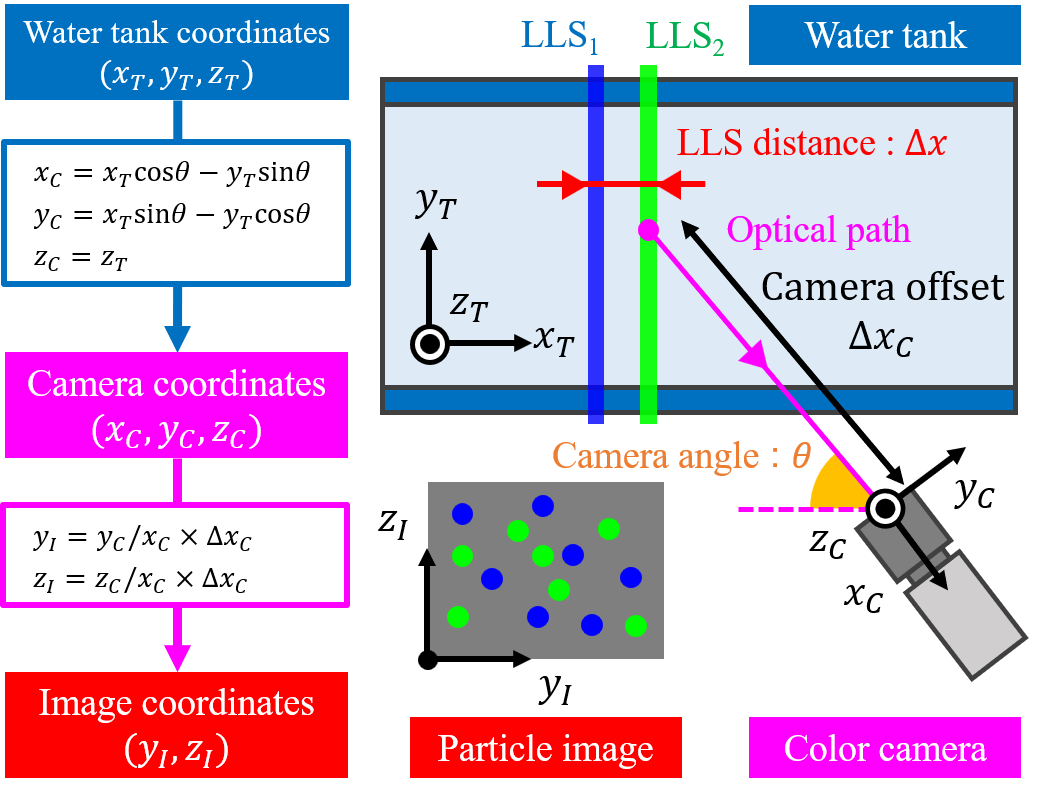
\includegraphics[keepaspectratio, width=80mm]{../images/Numerical_Simulation/Perspective_projection.png}
  \caption{Camera simulation model}
\end{figure}

\newpage
はじめに,水槽座標系における粒子像の位置 $(x_{Ti}, y_{Ti}, z_{Ti})$ ($i$は粒子番号) を
あらかじめ用意した任意の流れ場を用いて計算する.
次に,撮影角度 $\theta$ だけ回転したカメラ座標系における粒子像の位置
$(x_{Ci}, y_{Ci}, z_{Ci})$ を計算する.
最後に,透視投影の式を用いて画像座標系 $(y_{Ii}, z_{Ii})$ における粒子像の位置を計算し,
その位置を中心にガウス分布に従った輝度値を与えることで粒子像を生成することができる.
また,ぞれぞれの変換は以下の式で表すことができる.

\vskip 0.5 \baselineskip
\noindent $\blacksquare$ \textgt{水槽座標系からカメラ座標系への変換式}
\begin{eqnarray*}
  x_C &=& x_T \cos \theta - y_T \sin \theta \\
  y_C &=& x_T \sin \theta + y_T \cos \theta \\
  z_C &=& z_T
\end{eqnarray*}

\noindent $\blacksquare$ \textgt{カメラ座標系から画像座標系への変換式}
\begin{eqnarray*}
  y_I &= \frac{\Delta x_C}{z_C} y_C \\
  z_I &= \frac{\Delta x_C}{z_C} z_C
\end{eqnarray*}

\subsection{校正画像の生成}
ここでは,撮影シミュレーションモデルを用いて
実際に校正画像を作成する.
まず,校正点は3次元空間内に Fig.2 に示すように配置されている.
これらの点を数値シミュレーションのパラメータとして与え,
各座標位置を計算する.それぞれの計算過程で得られる座標位置を
Fig.3 に示す.

\begin{figure}[htbp]
  \centering
  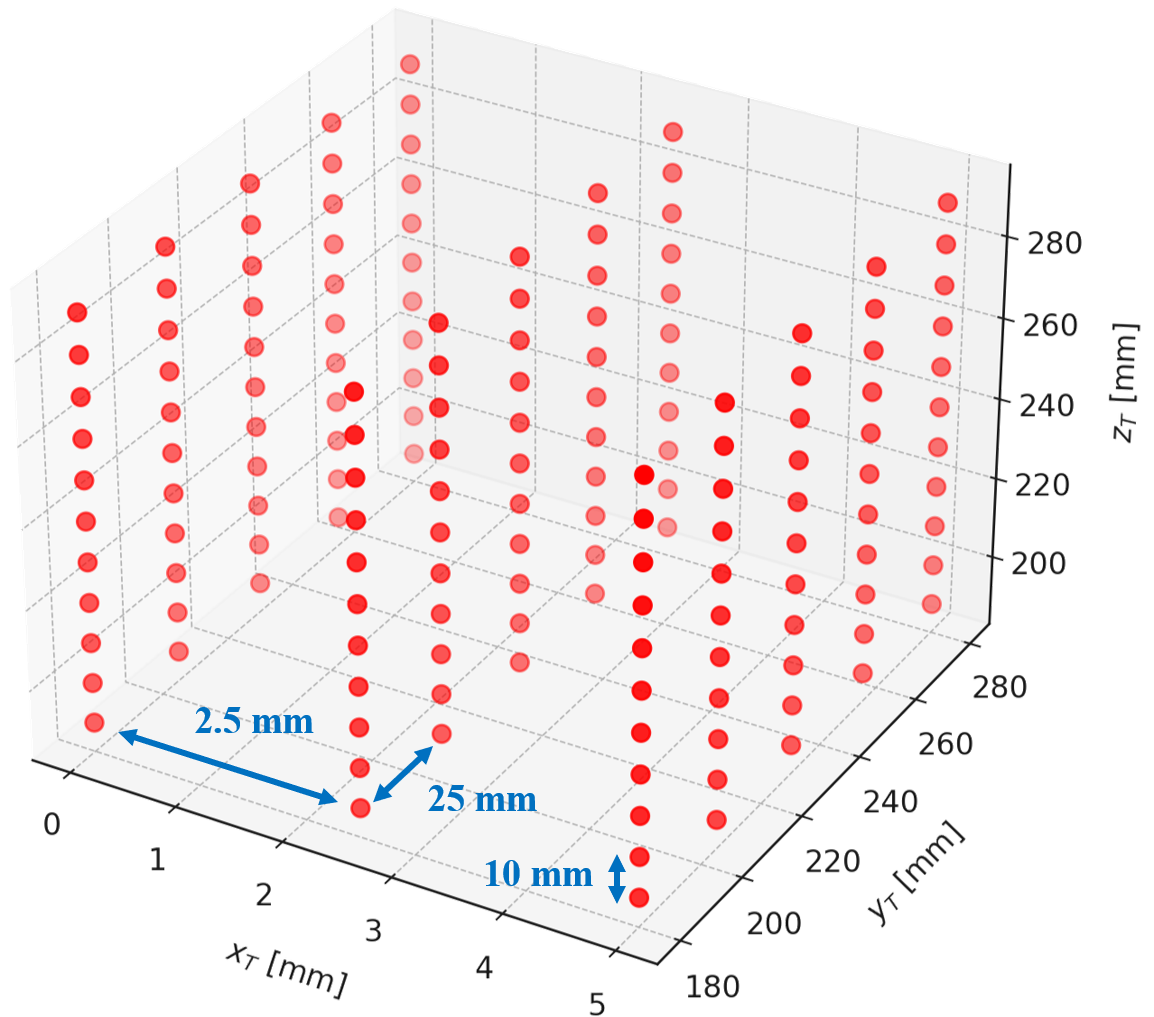
\includegraphics[keepaspectratio, width=70mm]{../images/Calibration/Calibration_points_in_3D_space.png}
  \caption{Calibration points in 3D space}
\end{figure}

\newpage
以上の画像における赤色の点が校正点の位置を表している.
また,(c) の画像座標系における校正点の位置から
作成した校正画像を Fig.4 に示す.

\begin{figure}[htbp]
  \centering
  {
    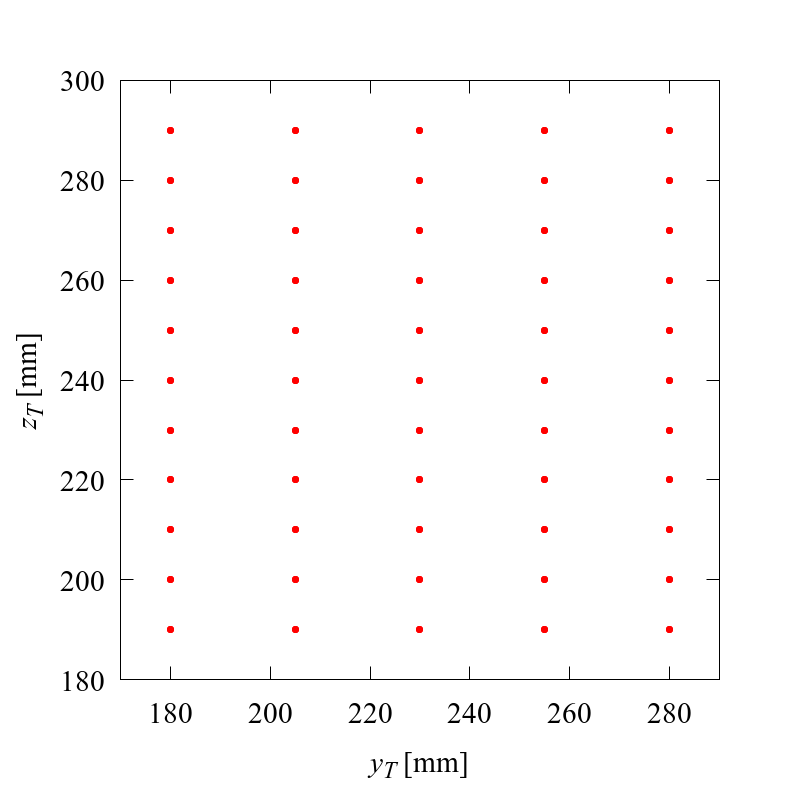
\includegraphics[keepaspectratio, width=72mm]{../images/Calibration/calibration_point_for_tank.png}
    \subcaption{Tank coordinates}
    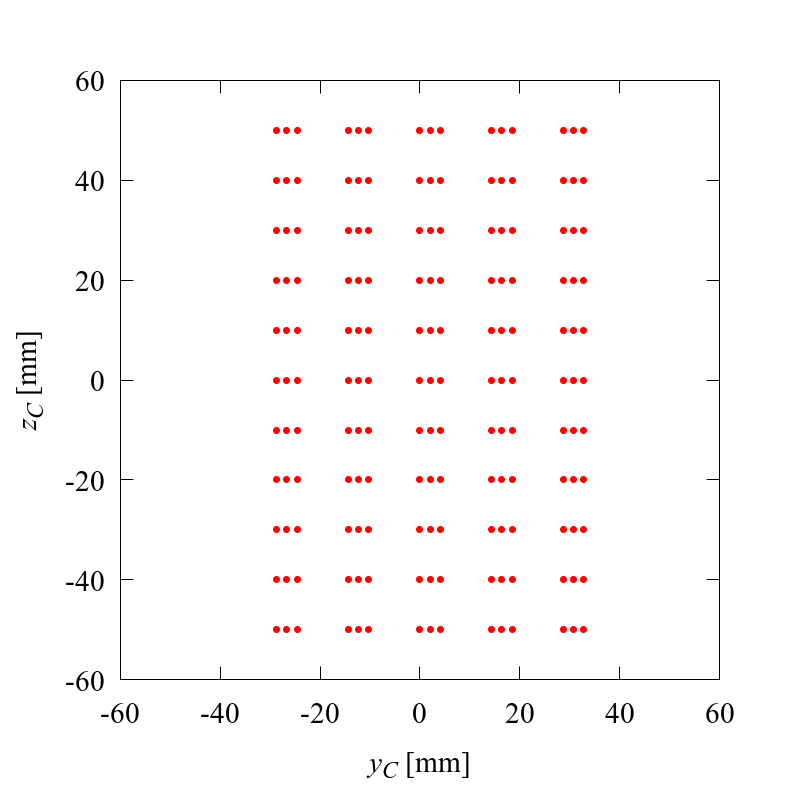
\includegraphics[keepaspectratio, width=72mm]{../images/Calibration/calibration_point_for_camera.png}
    \subcaption{Camera coordinates}
    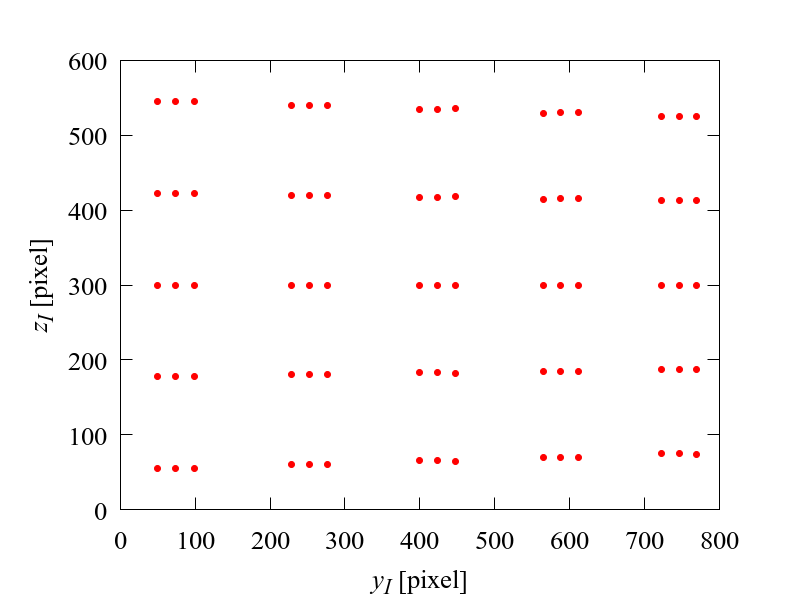
\includegraphics[keepaspectratio, width=72mm]{../images/Calibration/calibration_point_for_screen.png}
    \subcaption{Image coordinates}
  }
  \caption{Numerical simulation of calibration points}
\end{figure}

\begin{figure}[htbp]
  \centering
  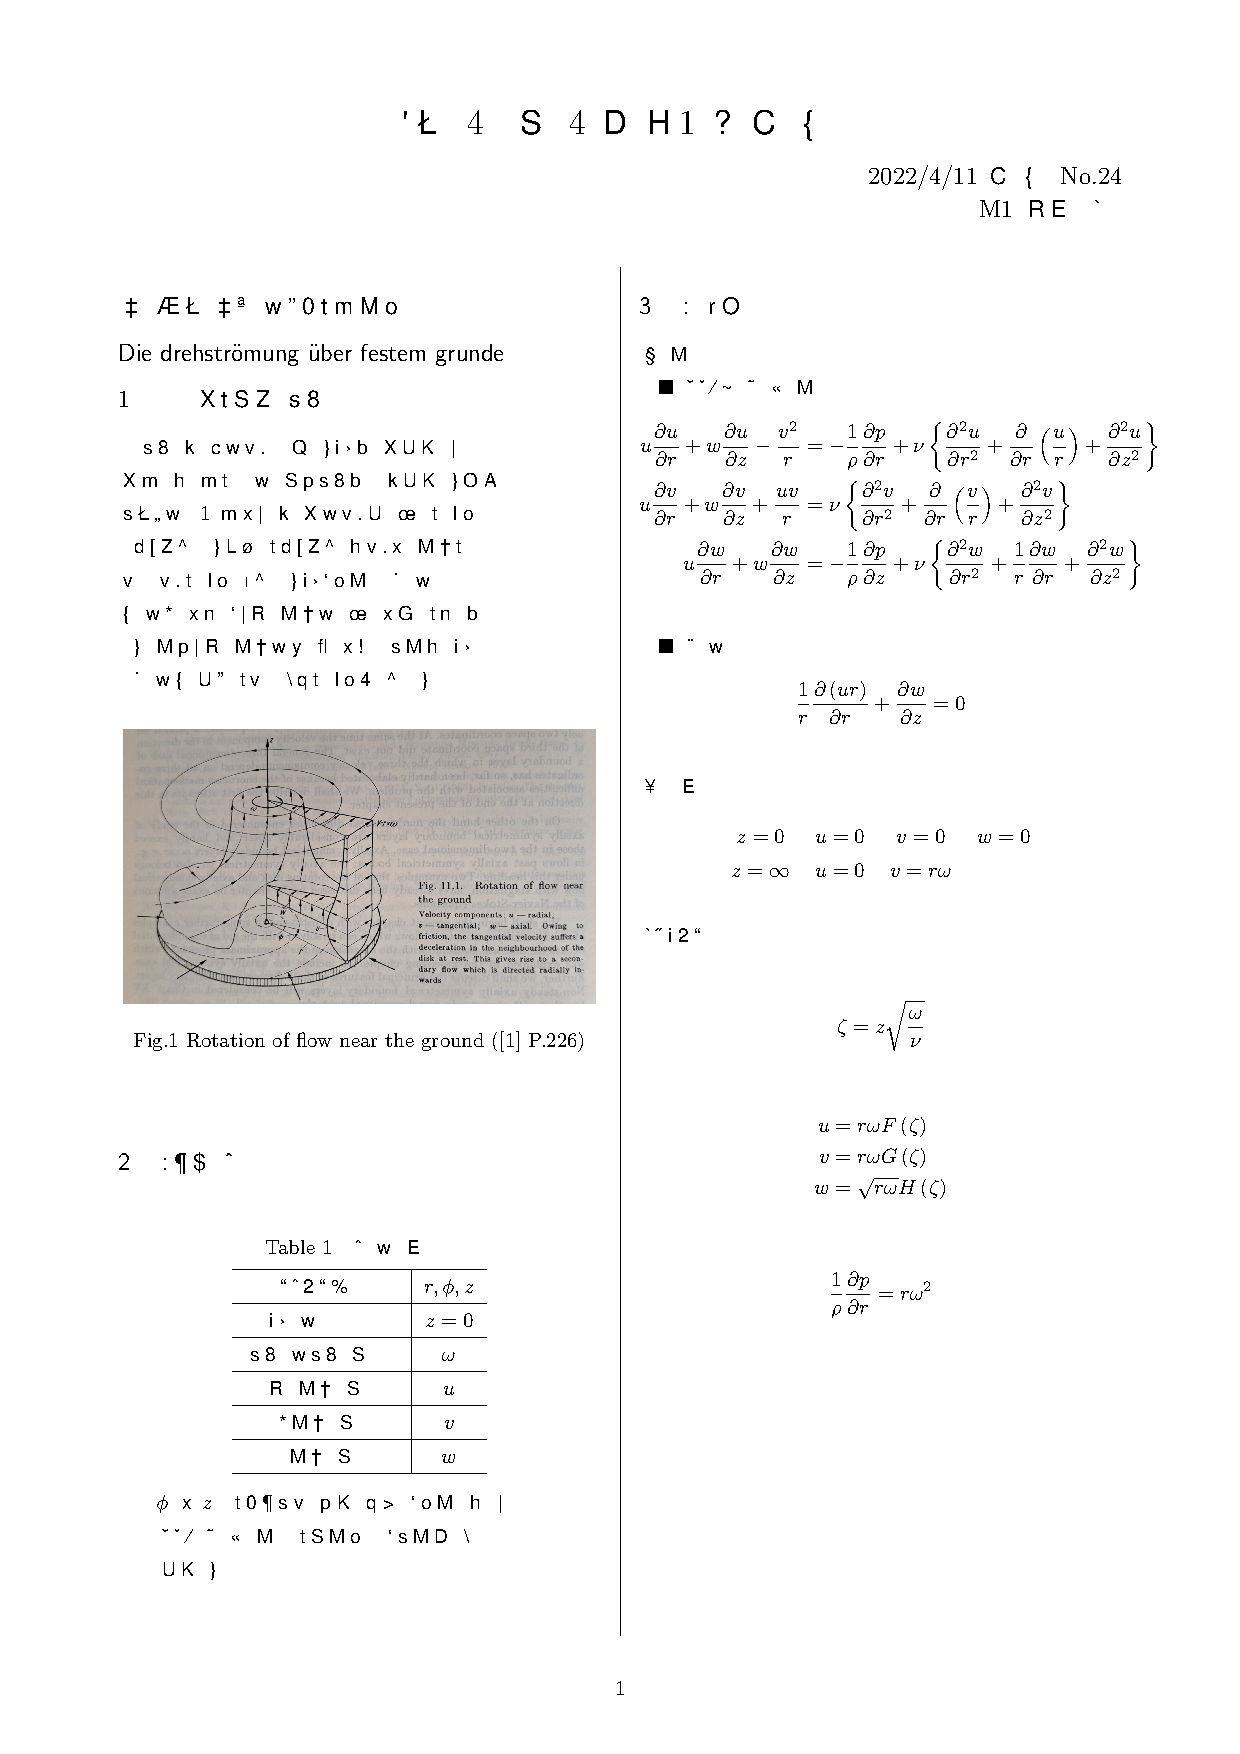
\includegraphics[keepaspectratio, width=60mm]{../images/Calibration/simulation.bmp}
  \caption{Calibration image created by camera simulation}
\end{figure}

\subsection{校正性能の数値的評価}
次に,作成した校正画像を用いて校正性能の評価する.
また,画像校正は以下の手順に従って行われる.

\begin{enumerate} [(1)]
  \item [$\blacksquare$] \gt{画像校正のプロセス}
  \item \gt{校正点の検出}
  \item \gt{校正式の取得}
  \item \gt{校正式を利用した画像変換}
\end{enumerate}

\subsubsection{校正点の検出方法と検出精度}
Fig.5 に示すように,粒子位置を粒子マスク相間法を用いて
相間平面を計算し,そのピーク値を粒子を中心として採用する.
位置の検出はサブピクセル精度で取得することができ,
粒子位置の検出精度を調べた結果を以下の Table 1 に示す.
また,粒子位置の検出についても同様の方法で行うことができる.

\begin{figure}[htbp]
  \centering
  \begin{tabular}{c c c}
    \begin{minipage}[t]{0.32\hsize}
      \centering
      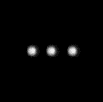
\includegraphics[keepaspectratio, width=25mm]{../images/Calibration/original.png}
      \subcaption{Original}
    \end{minipage}  &
    \begin{minipage}[t]{0.32\hsize}
      \centering
      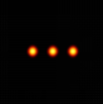
\includegraphics[keepaspectratio, width=25mm]{../images/Calibration/cross_crr.png}
      \subcaption{Cross-correlation}
    \end{minipage} &
    \begin{minipage}[t]{0.32\hsize}
      \centering
      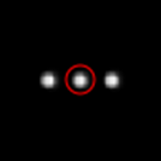
\includegraphics[keepaspectratio, width=25mm]{../images/Calibration/detection.png}
      \subcaption{Position}
    \end{minipage}
  \end{tabular}
  \caption{Calibration point detection}
\end{figure}

\begin{table}[hbtp]
  \centering
  \caption{RMSE of calibration point detection}
  \begin{tabular}{c r l r l}
    \hline
    $y_C$    & 0.579967 & pixel & 0.072496 & \% \\ \hline
    $z_C$    & 0.472066 & pixel & 0.078678 & \% \\ \hline
    $y_Cz_C$ & 0.747803 & pixel & 0.074780 & \% \\ \hline
  \end{tabular}\\
  \vskip 0.5 \baselineskip
  ※ 誤差率は変換前の画像サイズ$800\times600$を基準に計算
\end{table}

校正点の検出精度について,画像の横($y$)方向および縦($z$)方向における誤差率は
どちらも 0.07 \% 程度であり,十分な精度で検出することができており,
校正点検出および粒子検出における計測精度に問題はないといえる.

\newpage
\subsubsection{校正式の取得}
検出した校正点を用いて校正式を取得する.
校正式の取得は,Python の Scipy パッケージを用いて
多項式フィッティングを行うことで行うことができる.
ここでは,以下の2次元多項式を用いた校正式を採用している.
\vskip 0.5 \baselineskip
\noindent $\blacksquare$ \textgt{画像校正式}
\begin{eqnarray*}
  y_I &=& a_y y_C^3 + b_y y_C^2 z_C + c_y y_C z_C^2 + d_y z_C^3 + e_y y_C^2\\
  &+& f_y y_C z_C + g_y z_C^2 + h_y y_C + i_y z_C + j_y\\
  z_I &=& a_z y_C^3 + b_z y_C^2 z_C + c_z y_C z_C^2 + d_z z_C^3 + e_z y_C^2\\
  &+& f_z y_C z_C + g_z z_C^2 + h_z y_C + i_z z_C + j_z
\end{eqnarray*}
※ $y, z$ はカメラ座標系における座標位置を表し,
$z_I, y_I$ は画像座標系における座標位置を表す.

\vskip 0.5 \baselineskip
\subsubsection{校正式を利用した画像変換}
最後に,上述の校正式を利用して画像変換を行う.
実際に Fig.4 の画像に校正式を適用した結果を Fig.6 に示す.
ただし,校正は左列 ($x = 0 \rm{mm}$) の校正点を基準にした結果である.
また,画像変換精度の評価結果を Table 2 に示す.

\begin{figure}[htbp]
  \centering
  \includegraphics[keepaspectratio, width=70mm]{../images/Calibration/0.bmp}
  \caption{Calibrated image}
\end{figure}

\begin{table}[hbtp]
  \centering
  \caption{RMSE of RMSE of image calibration}
  {
    \subcaption{$x = 0.0\;\rm{mm}$}
    \begin{tabular}{c r l r l}
      \hline
      $y_I$    & 0.192323 & pixel & 0.024040 & \% \\ \hline
      $z_I$    & 0.169439 & pixel & 0.052950 & \% \\ \hline
      $y_Iz_I$ & 0.256316 & pixel & 0.029748 & \% \\ \hline
    \end{tabular}\\
    \vskip 0.5 \baselineskip
    \subcaption{$x = 2.5\;\rm{mm}$}
    \begin{tabular}{c r l r l}
      \hline
      $y_I$    & 0.192323 & pixel & 0.024040 & \% \\ \hline
      $z_I$    & 0.192891 & pixel & 0.060278 & \% \\ \hline
      $y_Iz_I$ & 0.272388 & pixel & 0.031613 & \% \\ \hline
    \end{tabular}\\
    \vskip 0.5 \baselineskip
    \subcaption{$x = 5.0\;\rm{mm}$}
    \begin{tabular}{c r l r l}
      \hline
      $y_I$    & 0.165201 & pixel & 0.020650 & \% \\ \hline
      $z_I$    & 0.150000 & pixel & 0.046875 & \% \\ \hline
      $y_Iz_I$ & 0.223139 & pixel & 0.025897 & \% \\ \hline
    \end{tabular}\\
  }
  \vskip 0.5 \baselineskip
  ※ 誤差率は変換後の画像サイズ$800\times320$を基準に計算
\end{table}
\newpage
画像変換精度の評価結果より,それぞれの誤差率は
$y_I$ が 0.02 \% 程度,$z_I$ が 0.05 \% 程度であり,
画像上座標系における$z_I$方向にやや大きな誤差を持つことがわかる.
しかし,これらの誤差は画像サイズに対して非常に小さな値であり,
画像校正の過程に問題はないといえる.

\section{一様流の数値シミュレーション}
画像校正における大きな問題点はないと考えれられるため,
撮影シミュレーションによって評価を行う.
今回は,一様流を模した流れ場から粒子像を作成し,
計測アルゴリズムの適用を行った.
また,撮影シミュレーションに用いた一様流は
$x_T$ 方向の流れ $u = 250\;\rm{mm/s}$ のみを考慮した流れ場である.
\vskip 0.5 \baselineskip

\subsection{撮影シミュレーションによる粒子像}
撮影シミュレーションによって作成した粒子像のオバーラップ画像を Fig.7 に示す.
これは,10枚分の画像を重ね合わせたものであり,一様流であることから
左から右方向に向かって粒子が移動していく様子が確認できる.

\begin{figure}[htbp]
  \centering
  \includegraphics[keepaspectratio, width=70mm]{../images/UniformFlow/UniformFlow_by_Simulation.bmp}
  \caption{Overlap of particle images ($n = 10$)}
\end{figure}

\subsection{計測アルゴリズムの適用結果}
実際に計測アルゴリズムの適用結果を Fig.8 に示す.
結果より,一様流の観測結果であるはずの流れ場が
一様に右方向に向かっていることが確認できる.
したがって,計測アルゴリズムに問題があることを確認した.

\begin{figure}[htbp]
  \centering
  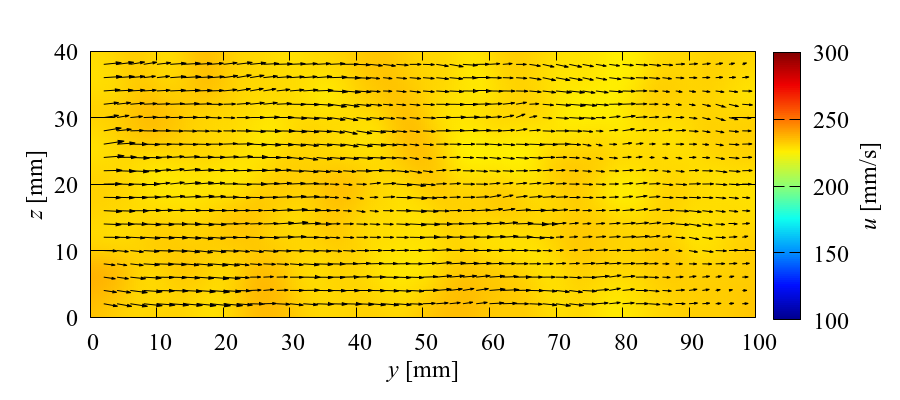
\includegraphics[keepaspectratio, width=85mm]{../images/UniformFlow/velocity_xyz.png}
  \caption{Time-averaged velocity}
\end{figure}


\end{document}